\documentclass[reprint,amsmath,amssymb,aps,prl]{revtex4-2}

\usepackage{dcolumn}% Align table columns on decimal point
\usepackage{bm}% bold math
\usepackage{graphicx} %LaTeX package to import graphics
\usepackage{siunitx}
\usepackage{hyperref}

\bibliographystyle{apsrev4-2}

\begin{document}

\title{Measuring Radiation Using a Geiger-Muller Counter}

\author{Gabriel Diaz-Espinoza}

\affiliation{The City College of New York}%

\date{\today}% It is always \today, today,

\begin{abstract}
A series of experiments using a Geiger-Muller counter was conducted on alpha, beta, and gamma radiation emitters. 
\end{abstract}

%\keywords{Suggested keywords}%Use showkeys class option if keyword
                              %display desired
\maketitle

%x\tableofcontents
\section{Experimental Setup and Procedures}
All of the experiments utilize the ST360 Radiation Counter with Geiger-Muller Tube (GM Tube) and stand (Counter box, power supply – transformer, GM Tube, shelf stand, USB cable, and a source holder for the stand) as shown in figure \ref{fig:st360_setup}. All radioactive sources are provided by Spectrum Technologies manufacturer, the specific isotope used is specified for each experiment. 
\begin{figure}
    \centering
    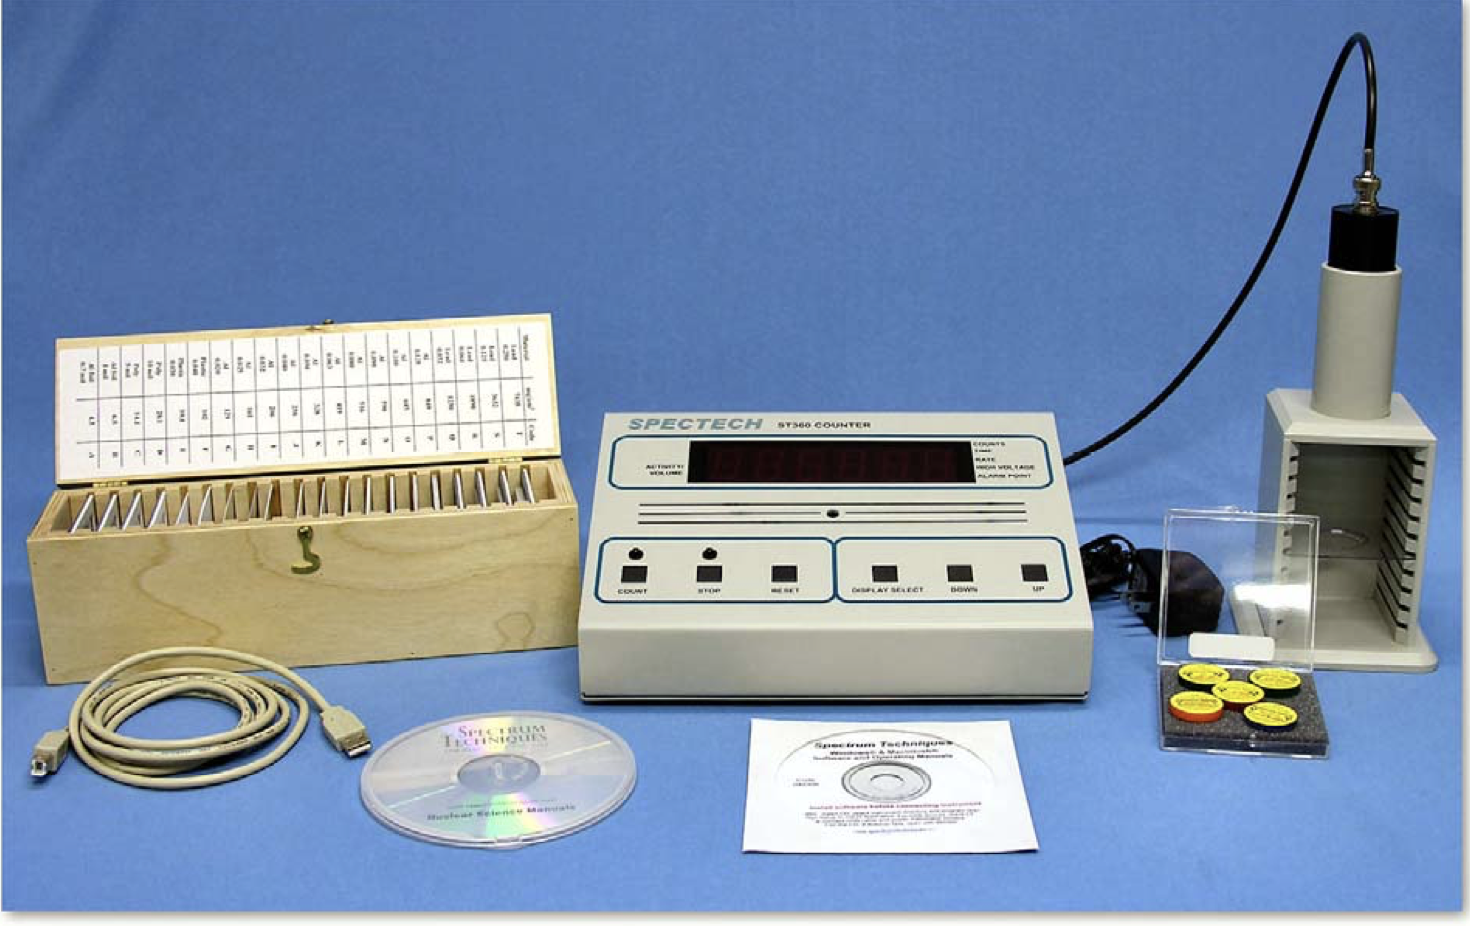
\includegraphics[scale = 0.2]{ST360_setup.png}
    \caption{ST-360 radiation counter with GM Tube and radioactive sources.}
    \label{fig:st360_setup}
\end{figure}

\section{Lab 1: Measuring GM Plateau}
\subsection{Introduction}
When radiation enters the GM tube, some of the gas atoms inside the tube will ionize. The positively charged ions and the negatively charged electrons will respond to the electric field inside the tube and they will travel to the cathode and anode, respectively. The electrons travel faster than the positively charged ions, and they ionize other atoms as they drift through the gas before reaching the anode. This ionization process produces what is referred to as a Townsend avalanche of electrons traveling in the tube towards the anode. The discharge current associated with this process causes the voltage between the anode and the cathode to drop. It is this voltage drop that is detected and is used to signal the presence of radiation particles. 

When the the radioactive sample is placed beneath the GM tube, and voltage in the tube is slowly ramped up, the counting does not begin immediately. There is a starting voltage where the "avalanche" can begin to produce a signal. As the voltage increases beyond this starting voltage, the the counting rate increases quickly before it stabilizes. Past this point of stabilization, commonly referred to as the "knee", small voltage increase leads to small increments in counting rate. This region of stability is known as the plateau. Increasing voltage beyond this region leads to a second large rise in counting rate. The region beyond the plateau is known as the "discharge" region. This experiment attempts to graphically show this plateau. 
\subsection{Experimental Setup and Procedure}
The ST-360 setup as shown in figure \ref{fig:st360_setup} was used. The radioactive source is Cs-137, as shown in figure \ref{fig: cs137}. 
\begin{figure}
    \centering
    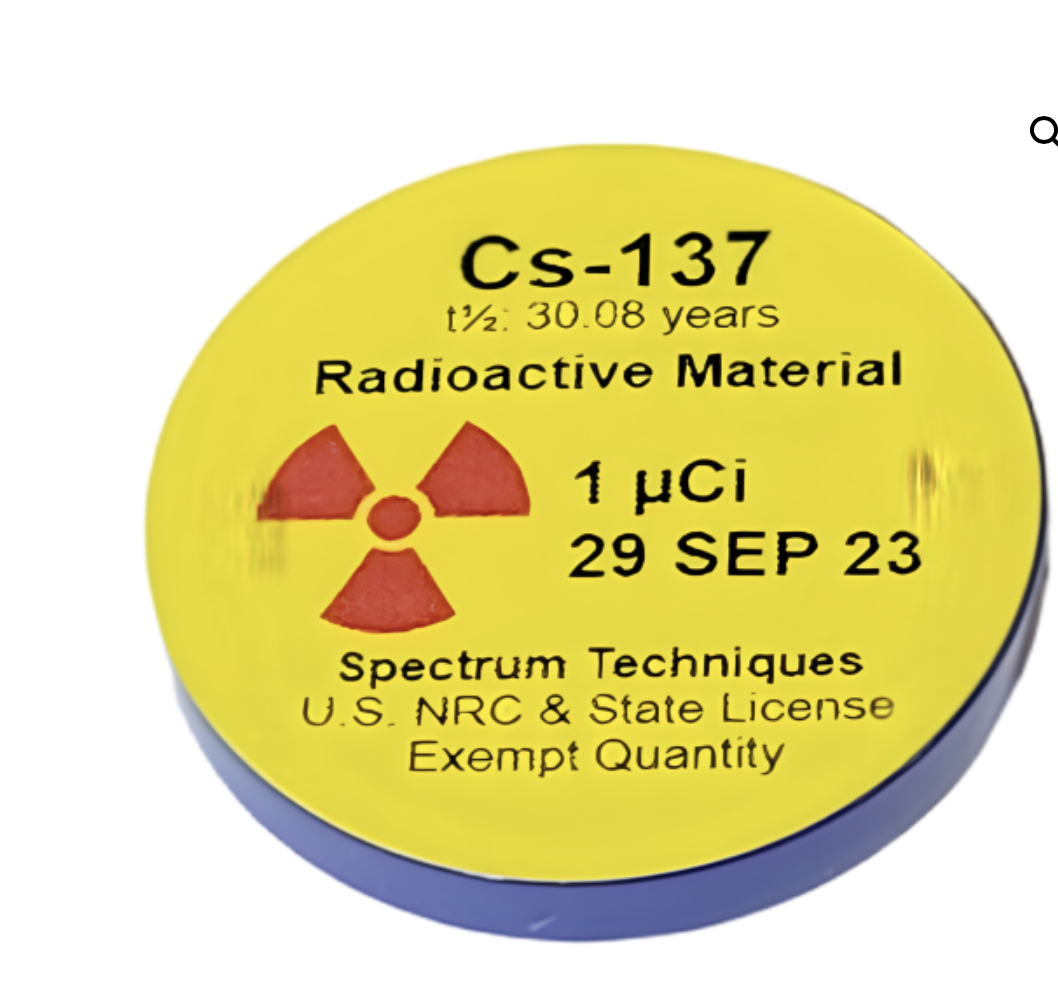
\includegraphics[scale = 0.1]{cs137.png}
    \caption{Cs-137 beta/gamma radiation disk source provided by Spectrum Technologies manufacturer.}
    \label{fig: cs137}
\end{figure}
The starting voltage used was 700 V. Radiation counts were obtained for thirty seconds before the voltage was increased by 20 V. Radiation counts were then obtained for thirty seconds for this new voltage and so forth. This process was repeated a total of twenty six times, such that the final voltage was 1200 V. The measurements were recorded onto a data file and analyzed. 

\subsection{Results}
A plot of the radiation counts is shown as a function of voltage in figure \ref{fig:gm_plateau}. There appears to be a very limited plateauing effect in the plot, the plot shows that the counts are always increasing. The shape of the graphs shows that the slope, while positive, does decrease at some point, before increasing again, demonstrating that a weak plateauing effect was observed. 
\begin{figure}
    \centering
    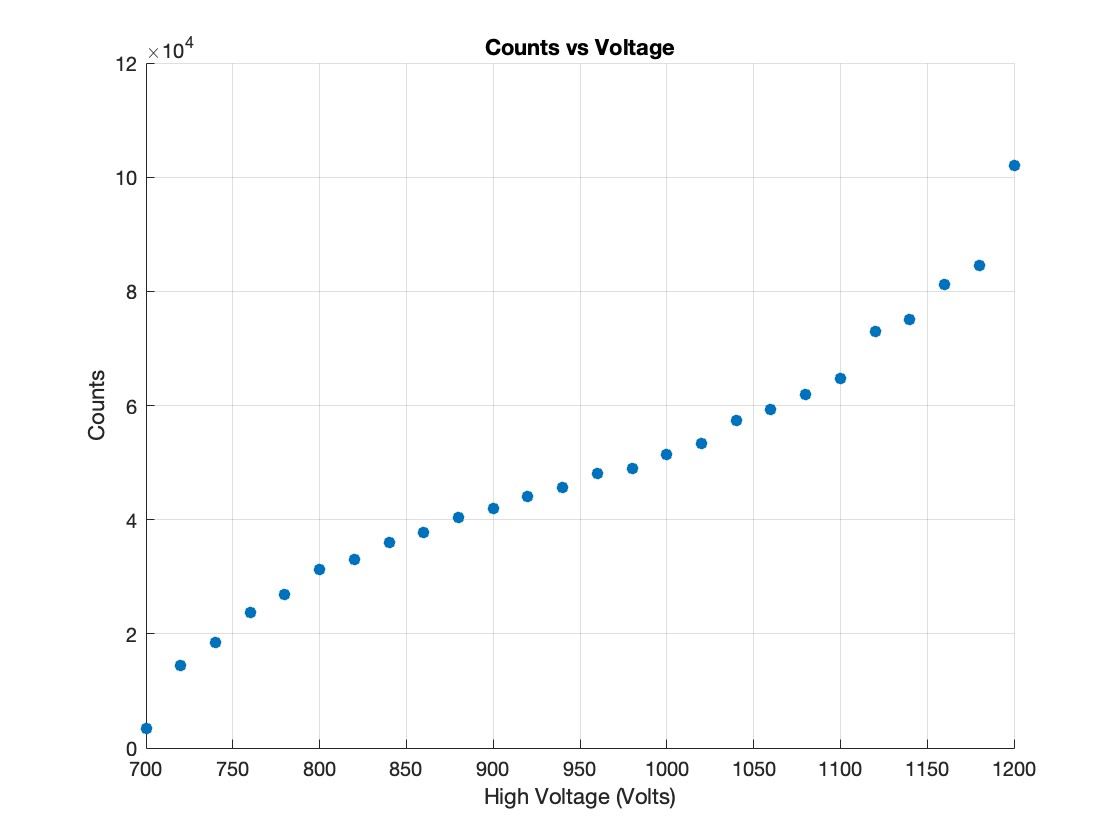
\includegraphics[width = \columnwidth]{GMPlateau.jpg}
    \caption{Plot of radiation counts as a function of voltage. The counts at a given voltage were performed for thirty seconds each.}
    \label{fig:gm_plateau}
\end{figure}
\subsection{Conclusions}
The plateauing effect as described in the introductory section of this lab was not observed. This can be due to systematic errors in obtaining the measurement of the counting rate such as not calibrating the GM tube properly. 

\section{Lab 2: Statistics of Counting }
\subsection{Introduction}
The radiation counter counts the number of radiation particles it detects in the GM tube at a given time. The amount of particles detected is often very large. As such, statistical methods must be used to deal with each particle simultaneously. A measurement counts the number of successes resulting from a given number of trials. A trial is assumed to have two possible outcomes: a success or not a success. For the Cs-137 isotope used in this experiment, the probability of decay (success) and non-decay is constant at every time. A measurment for this experiment consists of measuring radiation counts during a given interval of time. This experiment aims to use statistical methods to analyze the frequency of these counts across many measurements. 

\subsection{Experimental Setup and Procedure}
The ST-360 setup shown in figure \ref{fig:st360_setup} was used. The radioactive source is Cs-137, as shown in figure \ref{fig: cs137}. 
The voltage in the GM tube is 900 V. 

The first part of the experiment involved measuring the background radiation, with no radioactive source placed under the GM tube. A run for this part of the experiment involved measuring the background radiation (recording the number of counts) for five seconds. There were 150 runs.

The second part of the experiment involved measuring the radiation from Cs-137. The Cs-137 was placed under the GM tube. A run for this part of the experiment  involved measuring the radiation from the source (by recording the number of counts) for one second. There were 750 runs. 

\subsection{Results}
A plot of counts vs frequency for part.1 is shown in \ref{lab2_part1}. The predictions of the Gaussian and the Poisson distributions plotted using the data is also shown. The mean was calculated as $20.4$. The standard deviation was calculated to be 4.03. Curve fitting using builtin Matlab fit functions gave a mean of 18 for the distributions, and a standard deviation of 7.36 for the Gaussian distribution and a standard deviation of 4.24 for the Poisson distribution. As seen in the figures, plots of the Poisson and Gaussian distributions are very similar to each other. 

A plot of counts vs frequency for part 2 is shown in \ref{lab2_part2}. The predictions of the Gaussian and Poisson distributions plotted using the data is also shown. The mean was calculated as $1400$ and the standard deviation was calculated as 20.19. The mean for the Gaussian and Poisson distribution fits is 1385.5. The standard deviation of the Gaussian was found to be $38.83$. The standard deviation of the Poisson distribution was found to be $37.22$. The  values for both of these fits are in range with the calculated values of mean and standard deviation from the data. 


\begin{figure}
    \centering
    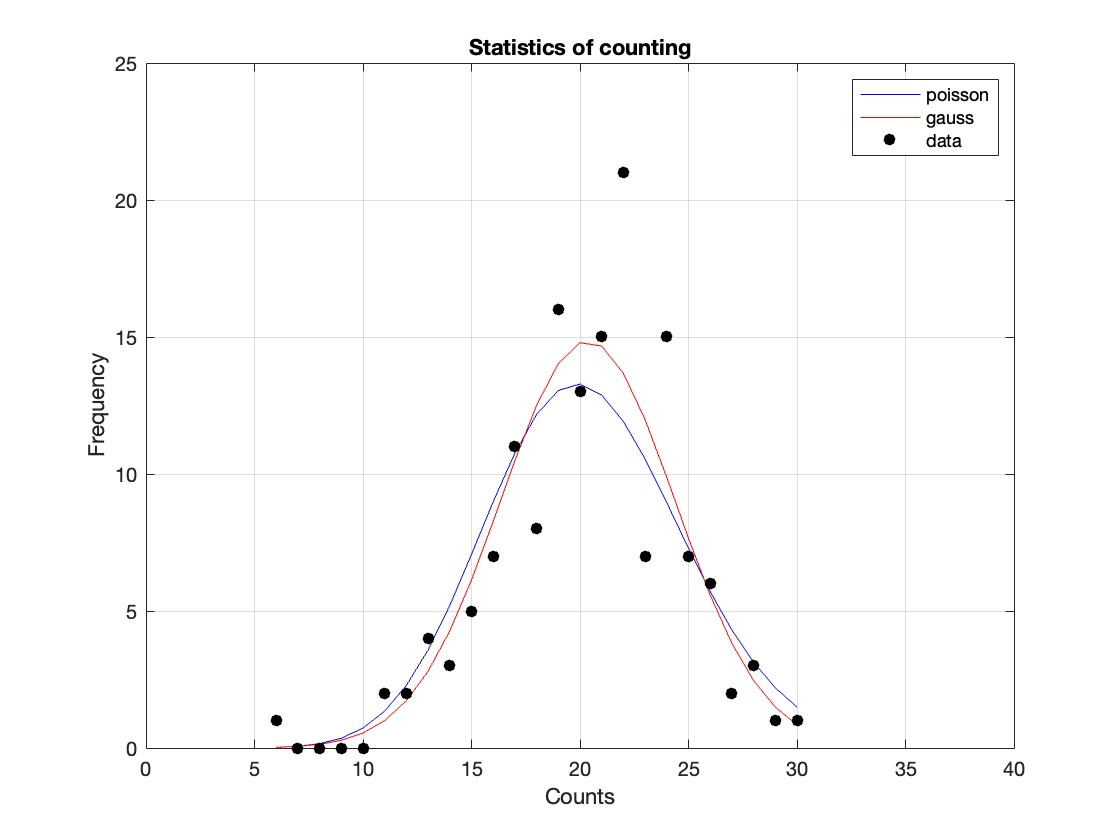
\includegraphics[width = \columnwidth]{lab2_part1.jpg}
    \caption{Plot of count frequencies for background radiation.}
    \label{fig:lab2_part1}
\end{figure}


\begin{figure}
    \centering
    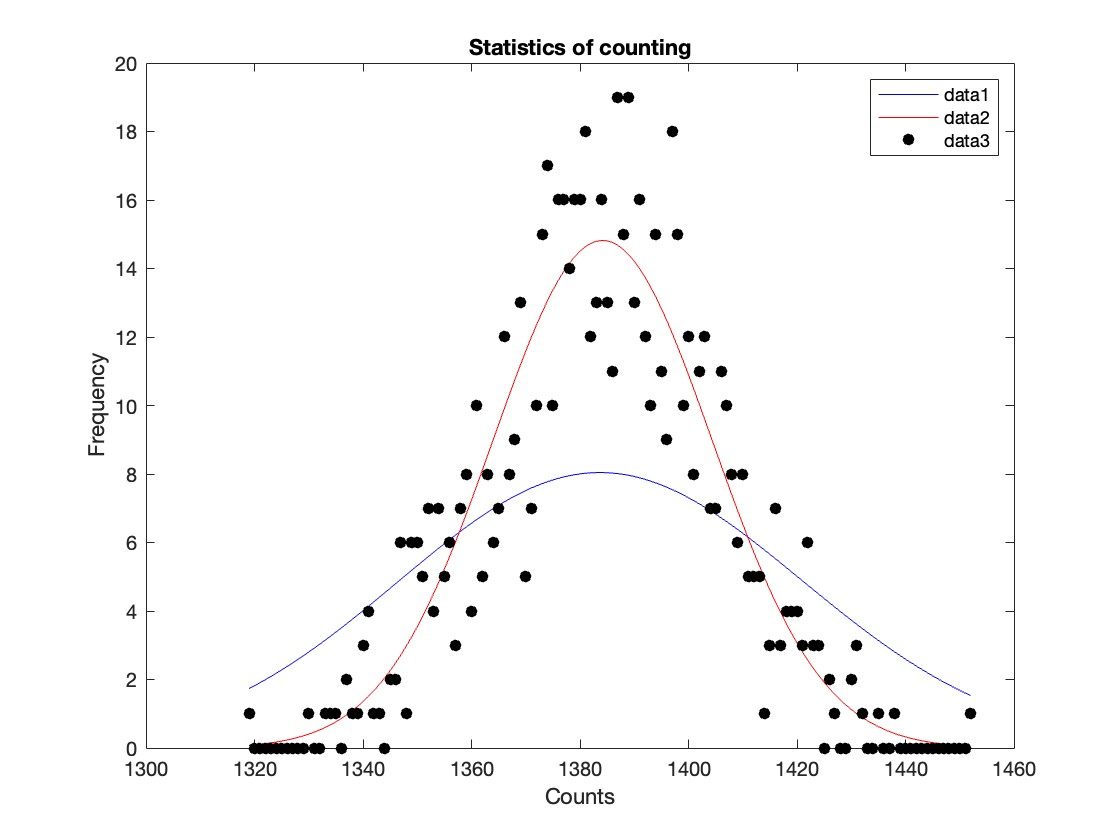
\includegraphics[width = \columnwidth]{lab2_part2.jpg}
    \caption{Plot of count frequencies for Cs-137 source.}
    \label{fig:lab2_part2}
\end{figure}

\subsection{Conclusions}
The Poisson and the Gaussian distributions are distributions that describe the behavior of the counting rate measurements. For the second part of the experiment, the Poisson distribution does not describe the behavior very well, but the Gaussian distribution remains useful. 

\section{Lab 3: Background Radiation }

\subsection{Introduction}
The GM tube is bombarded by radiation even when there is no radioactive isotope like Cs-137 present. This leads to an overestimate of radiation counts whenever measuring the radioactivity of an isotope. In this experiment, we learn to compensate background radiation by subtracting the radiation counts when no isotope is present from the radioactivity measurement of an isotope sample. 

\subsection{Experimental Setup and Procedure}
The The ST-360 setup as shown in figure \ref{fig:st360_setup} was used. The
radioactive source is Cs-137, as shown in figure \ref{fig: cs137}. The operating voltage is 900 V. The background radiation was measured by recording the number of counts in a five-minute interval. The measurements were recorded for three such intervals. The Cs-137 sample was then placed under the GM tube and radiation counts were recorded for three runs of five-minute intervals each. MATLAB was then used to provide an estimate of the average radiation counts per five minute interval, correcting for background radiation. 

\subsection{Results}
Figure \ref{fig:lab3_background_table} displays a table of the background radiation counts for the experiment. The average background count per five minute interval is 1319  +/- 32.9 counts. 

Figure \ref{fig:lab3_cs137_table} displays a table of the raw radiation counts for the Cs-137 sample. The average raw count in a five minute interval is 418979 +/- 638.9. 

The true counts for a five minute interval is calculated by subtracting the average background counts from the average raw counts. The estimated average true counts for the radioactivity of the Cs-137 sample in a five minute interval is 417660 +/- 605.9. 

\begin{figure}
    \centering
    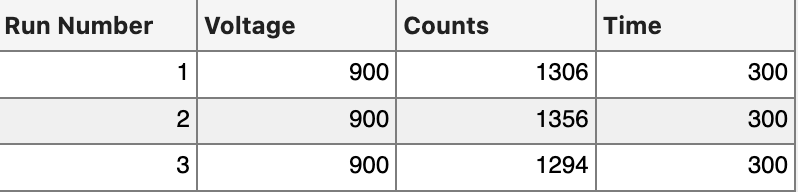
\includegraphics[width = \columnwidth]{lab3_background_table.png}
    \caption{Background radiation counts for Lab 3.}
    \label{fig:lab3_background_table}
\end{figure}
\begin{figure}
    \centering
    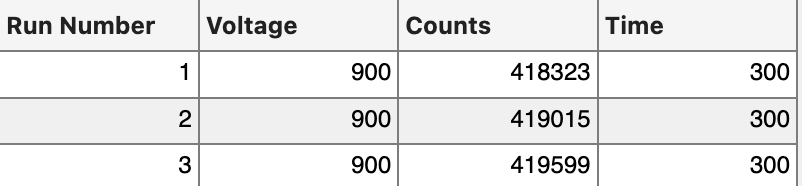
\includegraphics[width = \columnwidth]{lab3_cs137_table.png}
    \caption{Cs-137 radiation counts for Lab 3.}
    \label{fig:lab3_cs137_table}
\end{figure}

\subsection{Conclusions} 
The background radiation is not high compared to a radioactive source. In fact, the average background radiation is only about 0.32 $\%$  as large as the estimated true radiation counts. Nonetheless, it is useful to account for background radiation in obtaining measurements from isotopes. While the background radiation is trivial compared to radioactive sources, the background counts per year for example, would be an estimated 139 million counts. It is important to account for such numbers whenever measuring radiation for prolonged periods of time. 


\section{Lab 5: Geiger Tube Efficiency}
\subsection{Introduction}
The Geiger counter does not count all of the particles emitted from the radioactive source. One of the reasons why is because the radioactive source emits particles uniformly in all directions, and not all the particles enter the GM tube. 
The objective of the experiment is to find the efficiency of the GM counter by obtaining a measurement of the disintegration rate of various types of radioactive isotopes. 

A radioactive source emits particles at a constant rate which can be measured as disintegrations per minute (dpm). The GM counter measures counts per minute (cpm) which is equal to dpm because each disintegration represents an emitted particle. The radioactive isotope has an expected emission activity given by manufacturer specifications in microCuries ($\mu$Ci). The conversion factor is given as

\begin{equation*}
    1 \ \mu Ci =  \SI{2.22e6}{dpm.} = \SI{2.26e6}{cpm}
\end{equation*}
    
Using this conversion factor, the expected cpm of the source is found and compared to the cpm measured in experiment. The efficiency of the GM tube is found by comparing the percentage of counts observed versus the expected counts with the following equation:

\begin{equation} \label{lab5 percentage formula}
    \% \ \text{efficiency} = \frac{r(100)}{C K}
\end{equation}
where r is the measured activity in cpm, C is the expected activity in microCuries, and K is the conversion factor from microCuries to cpm.

 \subsection{Experimental Setup and Procedures}
The ST-360 setup shown in figure \ref{fig:st360_setup} was used. The voltage in the GM tube was set to 900 V. 

The efficiency of the GM tube was measured for three different sources of radiation. The sources used were alpha, beta and gamma radiation sources which correspond to samples of Po-210, Sr-90 and Co-60 respectively. 

The background cpm was measured first to account for over-counting due to background radiation. The radioactive source was then placed on a shelf below the GM tube, and counts were recorded for a minute to obtain a measurement of cpm for the source. 

\subsection{Results}
Figure \ref{fig:lab5_table} shows the efficiency of the GM tube when measuring radiation counts for different sources. The percent efficiency of the Sr-90 beta source of radiation is the highest by far.  
\begin{figure}
    \centering
    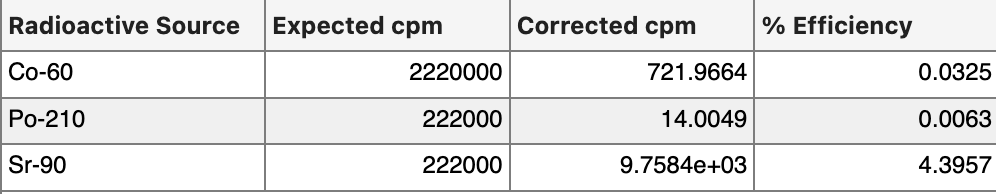
\includegraphics[width = \columnwidth]{lab5_table.png}
    \caption{Percent efficiency of Geiger Tube}
    \label{fig:lab5_table}
\end{figure}

\subsection{Conclusions}
The three different sources of radiation gave different measures for the efficiency of the GM tube. This is to be expected since the different radiation particles can travel at different velocities and scatter and disperse differently as a result. It would be ideal if this experiment can be conducted again, but using different shelves that are different distances away from the GM tube to observe how the efficiency would change for each isotope. It would be interesting to see if the alpha and/or gamma radiation source efficiencies can surpass that of the beta source.

\section{Lab 6: Shelf Ratios}
Whenever a radioactive source is placed under the GM tube, only a fraction of the radiation emitted by the source enters the GM tube to be counted. This fraction is a function of the distance $h$ from the point source to the GM tube. As figure \ref{fig:distanceFromTube} shows, the further away the source is from the GM tube window, the less radiation will enter the GM tube. This experiment seeks to confirm this observation by comparing the amount of measured radiation as the source moves further from the GM tube.

\subsection{Experimental Setup and Procedure}
The ST-360 setup in \ref{fig:st360_setup} is used. The voltage is 900 V. The radioactive source is Sr-90. A measurement of the background radiation is conducted. The radioactive source is then placed in the top shelf of the stand which is 2 cm away from the tube. The radiation counts are measured for thirty seconds. The radioactive source is then placed in the shelf below, and the counts are measured for thirty seconds. This process is repeated, moving down the shelves up to the tenth shelf. 

\subsection{Results}
Figure \ref{fig:lab6_shelf_ratios} shows the ratios between the counts in each shelf and the shelf 2 counts. Figure \ref{fig:lab6_plot} fits the data to a curve. The data is fit to a polynomial, where the fit is $y = 2.0851 x^{-0.7065} \ - \ 0.3279$. The fit demonstrates an inverse relationship between distance and radioactivity as expected. 

\begin{figure}
    \centering
    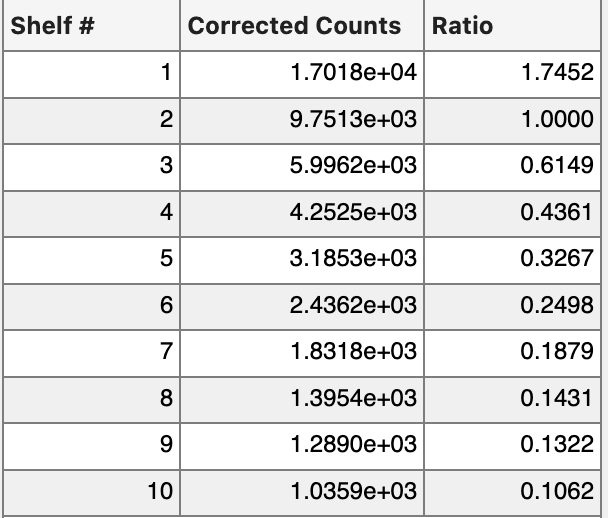
\includegraphics[width = \columnwidth]{lab6_shelf_ratios.png}
    \caption{Comparison of the radiation counts (corrected for background radiation) when source is in the second shelf to all other shelves. }
    \label{fig:lab6_shelf_ratios}
\end{figure}

\begin{figure}
    \centering
    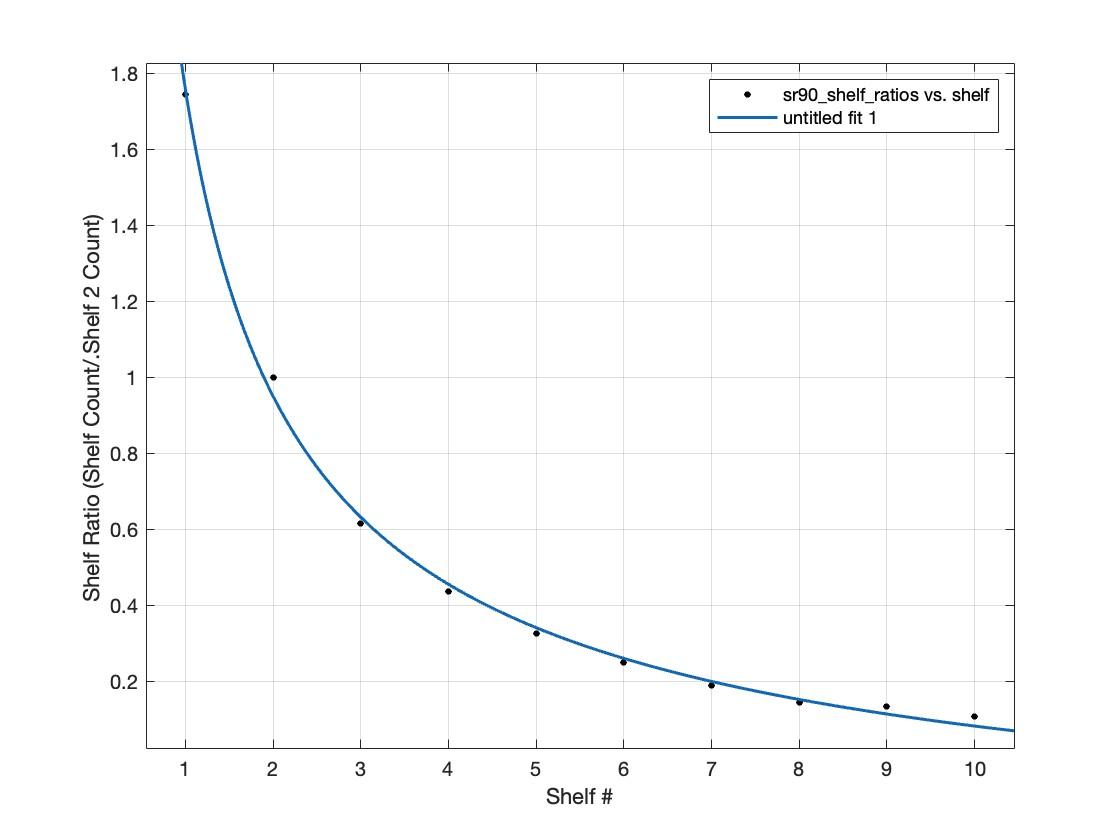
\includegraphics[width = \columnwidth]{Lab6_plot.jpg}
    \caption{Plot of shelf ratios seen in figure \ref{fig:lab6_shelf_ratios}. The data is fitted to a polynomial.}
    \label{fig:lab6_plot}
\end{figure}
\begin{figure}
    \centering
    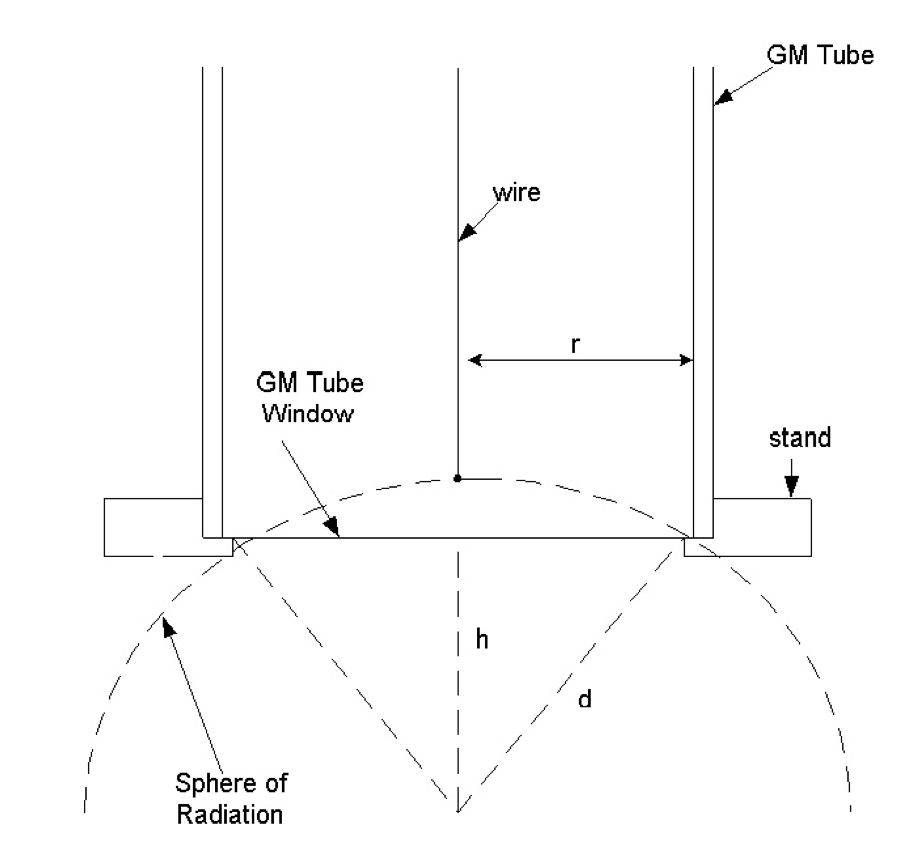
\includegraphics[width = \columnwidth]{DistanceFromTube.png}
    \caption{Relationship between distance from tube and observed counts. Credit: Spectrum Techniques Lab Manual}
    \label{fig:distanceFromTube}
\end{figure}
 \subsection{Conclusions} 
 There is a noticeable decrease in values as the source moves further away from the GM tube. It would be interesting to conduct an experiment to find and explicit relationship between the counting rate and distance from source. 

\section{Lab 7: Backscattering}
\subsection{Introduction}
For a sample placed under the radiation tube, most of the radiation is emitted away from the tube. Radiation strikes matter and is then scattered or deflected through varying angles. When the angle of deflection is approximately 180 degrees, the deflection is known as backscattering. For Geiger counters, backscatter is the fraction of radiation emitted away from the GM tube that strikes the material supporting the sample. It is deflected toward the tube window and is counted. 

The experiment seeks to measure the relationship between the aerial thickness of an absorber, measured in ($\frac{mg}{cm^2}), and backscattering. 

The  relationship between thickness and backscattering can be measured by calculating the percentage of the counts that are due to backscattering using the following: 
\begin{equation} \label{eq: lab7 percentage formula}
    \% \ \text{backscattering} = \frac{r - r_0}{r_0} \times 100 
\end{equation}
where $r$ is the corrected cpm and $r_0$ is the count rate without any absorber present. 
 
\subsection{Experimental Setup and Procedure}
The ST-360 setup is used and the operating voltage is 900 V.  The radiation source is a sample of the Sr-90 isotope. A measurement of the cpm due to background radiation is recorded. The Sr-90 is placed on the second shelf, with no absorber present, and the cpm is recorded. This measurement is used for comparison purposes. An aluminum absorber is then placed in the source holder on the second shelf and the source is placed directly above it. The radiation counts per minute is measured and recorded. The source is placed on an aluminum absorber that has a different thickness and the cpm is recorded. This procedure is done for a total of five different absorber thicknesses. 

\subsection{Results}
Figure \ref{fig:lab7_part2_plot} shows the relationship between absorber thickness and the backscattering percentage. Figure \ref{lab7_part2_plot.jpg} plots the corrected counts as a function of absorber thickness. There is a linear relationship between these two variables. The equation of the linear fit is counts = $ 3 \times$ thickness + 10425. 


\begin{figure}
    \centering
    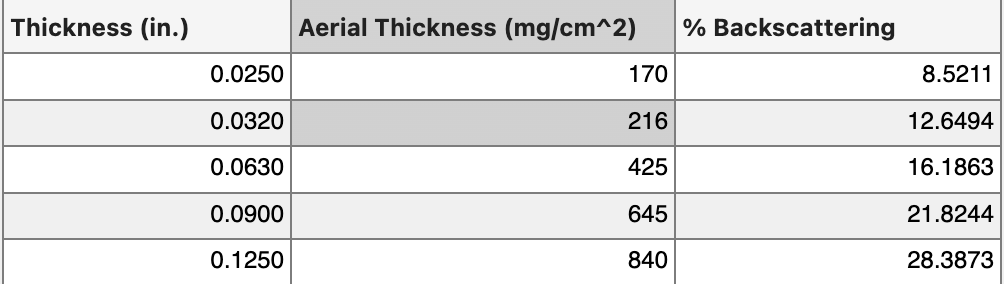
\includegraphics[width = \columnwidth]{lab7_al_thickness_table.png}
    \caption{Relationship between absorber thickness and backscattering}
    \label{fig:lab7_plot_absorber_thickness}
\end{figure}

\begin{figure}
    \centering
    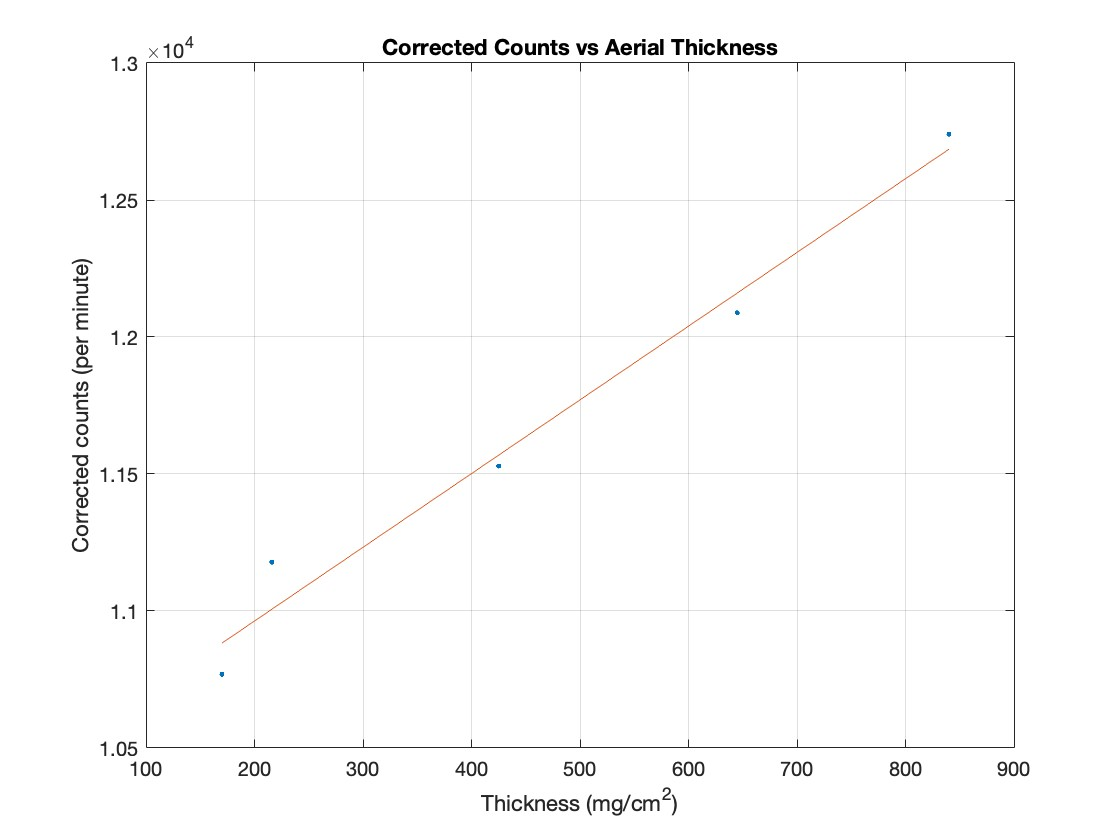
\includegraphics[width = \columnwidth]{lab7_part2_plot.jpg}
    \caption{Plot of corrected counts as a function of absorber thickness. The plot is fitted to a line.}
    \label{fig:lab7_part2_plot}
\end{figure}


\section{Lab 8: Inverse Square Law}

\subsection{Introduction}
As explained in Lab 6, the further away the source of radiation is from the GM tube, the lower the amount of radiation counted. Indeed, \ref{fig: distanceFromTube} suggests that there should be an inverse square relationship between the distance from the source and the intensity of radiation measured. This experiment seeks to verify that relationship.

\subsection{Experimental Setup and Procedure}
The ST-360 setup is used. The voltage is 900 V. The radioactive source is a sample of Sr-90 isotope.  The procedure is the same as that of Lab 6. A measurement of the background radiation is conducted. The radioactive source is then placed in the top shelf of the stand which is 2 cm away from the tube. The radiation counts are measured for thirty seconds. The radioactive source is then placed in the shelf below, and the counts are measured for thirty seconds. This process is repeated, moving down the shelves up to the tenth shelf. 

\subsection{Results}
Figure \ref{fig: lab8_plot} shows a linear relationship between $\text{(distance)}^{-2}$ and counts. The linear fit has the equation: $y = 6.7 x \ + \ 1055.1$. 



\begin{figure}
    \centering
    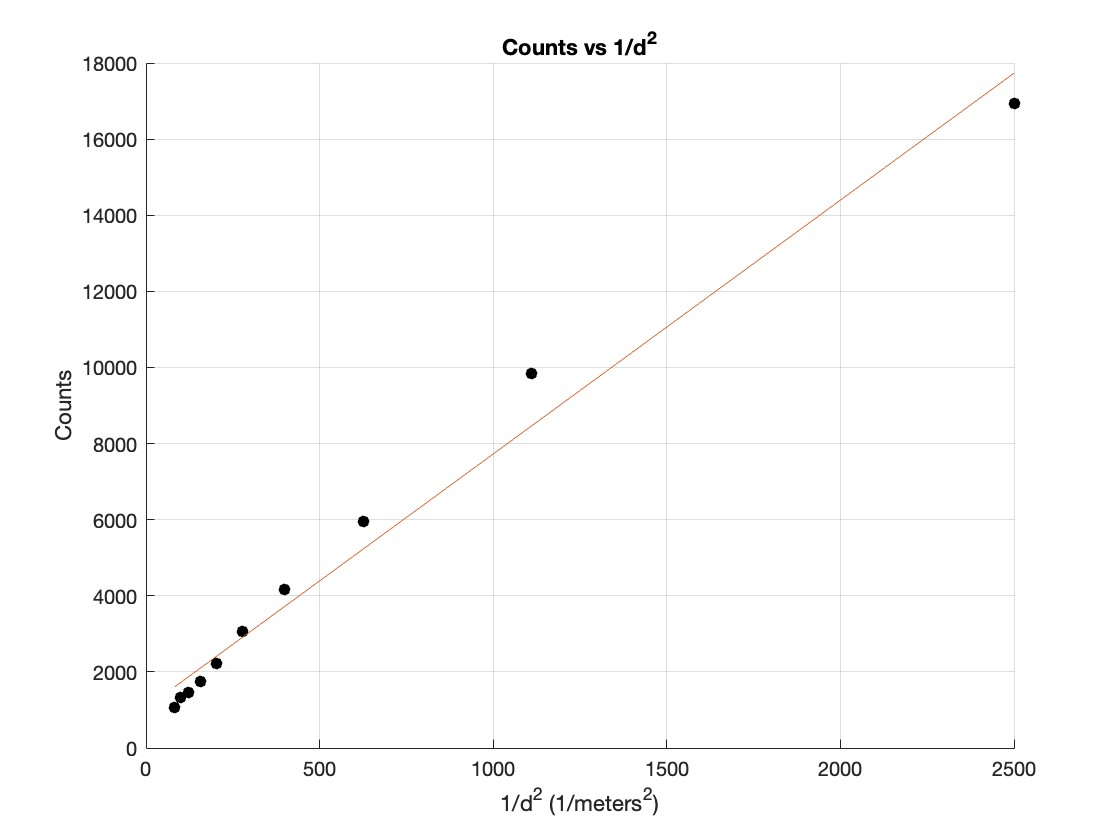
\includegraphics[width = \columnwidth]{lab8_plot.jpg}
    \caption{Plot of inverse square law relationship between corrected counts and distance from source to GM tube.}
    \label{fig: lab8_plot}
\end{figure}


\section{Lab 13: Half-Life of Ba-137m}
\subsection{Introduction}
A radioactive atom decays at a constant rate. If we know the number of atoms present and their decay constant (probability of decay per unit time), then the amount of atoms that remain at a given future time can be calculated using equation \ref{eq:lab13_first_equation} where $N(t)$ is the number of atoms present currently, $\lambda$ is the decay constant and $\Delta t$ is the elapsed time. 
\begin{equation} \label{eq: lab13_first_equation}
    N(t) = N - \lambda N \Delta t   
\end{equation}


\begin{figure}
    \centering
    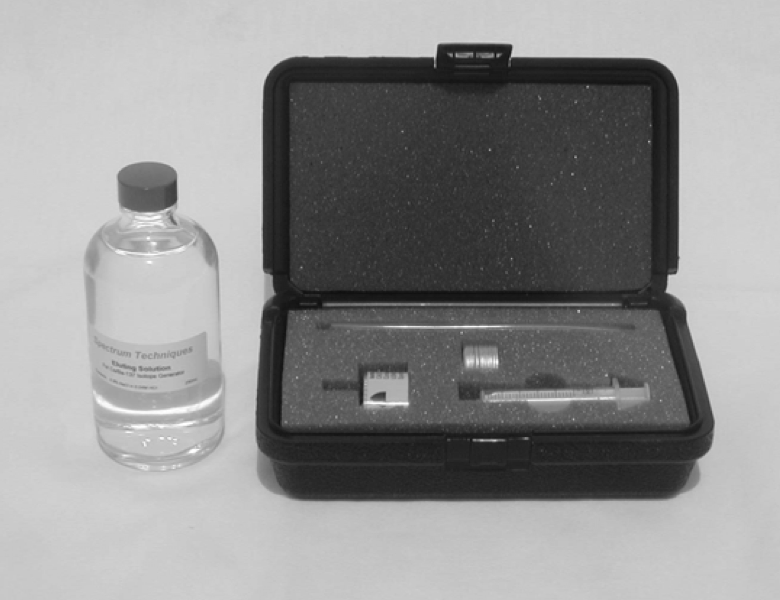
\includegraphics[width = \columnwidth]{IsotopeGenerator.png}
    \caption{Isotope Generator used to make Ba-137m from Cs-137m}
    \label{fig: IsotopeGenerator}
\end{figure}


The decay of radioactive atoms can be expressed in terms of the half-life. The observed activity of a sample detected by the Geiger counter is proportional to the number of radioactive atoms. Each count represents one atom decaying and releasing one particle or ray of radiation. As such, the activity is equal to the number of counts per unit of time which is equal to the number of atoms per unit of time. The half-life $t_{1/2}$ can be expressed as in equation \ref{eq: lab13 halfTime formula}. 

\begin{equation} \label{eq: lab13 halfTime formula}
    t_{1/2} = \frac{ \text{ln} (2)}{ \lambda }
\end{equation}


\subsection{Experimental Setup and Procedure}
The ST-360 setup is used with an operating voltage of 900 V. The radioactive source is Ba 137-m, obtained by using the Isotope Generator shown in figure \ref{fig: IsotopeGenerator}. The background radiation for a thirty-second interval is measured. From the isotope generator, Ten to twelve drops of Ba-137m are obtained. The radioactive source is then placed on the second shelf from the top. Thirty-one runs of obtaining radiation counts for thirty-second intervals were made.  


\subsection{Results}
\begin{figure}
    \centering
    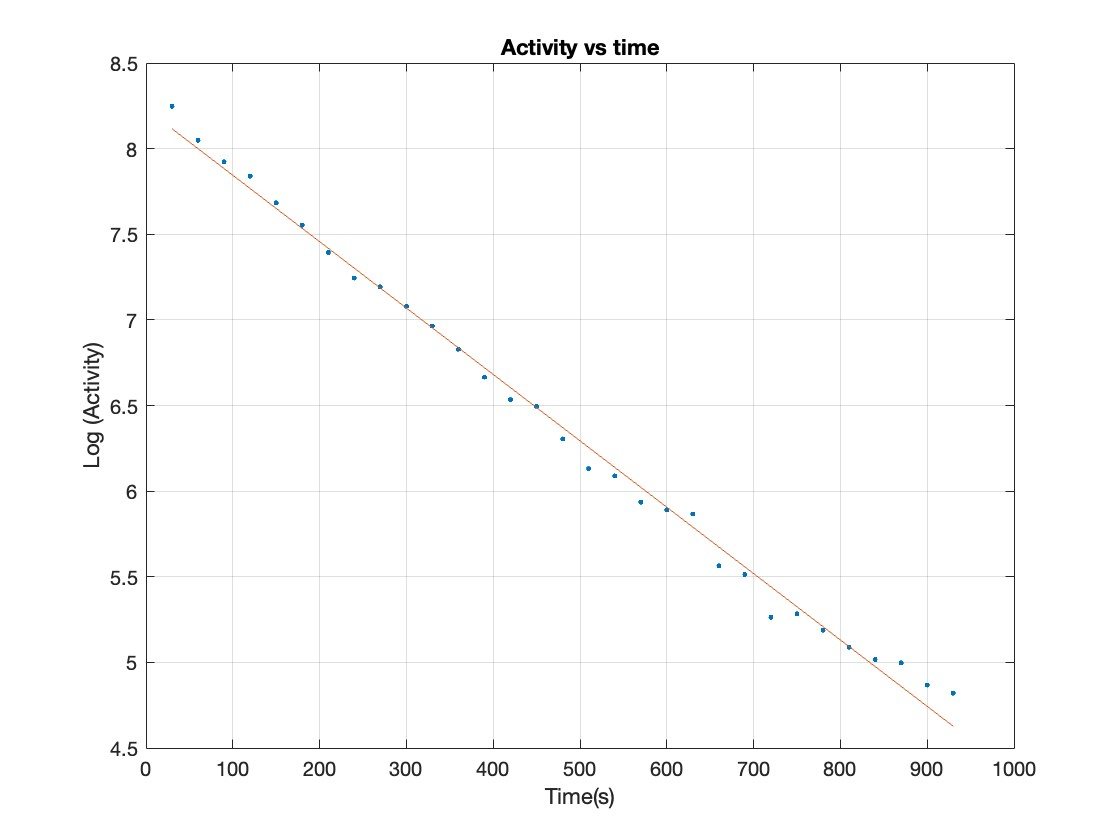
\includegraphics[width = \columnwidth]{Lab13_ActivityPlot.jpg}
    \caption{Plot of Ln(radiation counts) as a function of time}
    \label{fig: ActivityPlot_Lab13}
\end{figure}

\begin{figure}
    \centering
    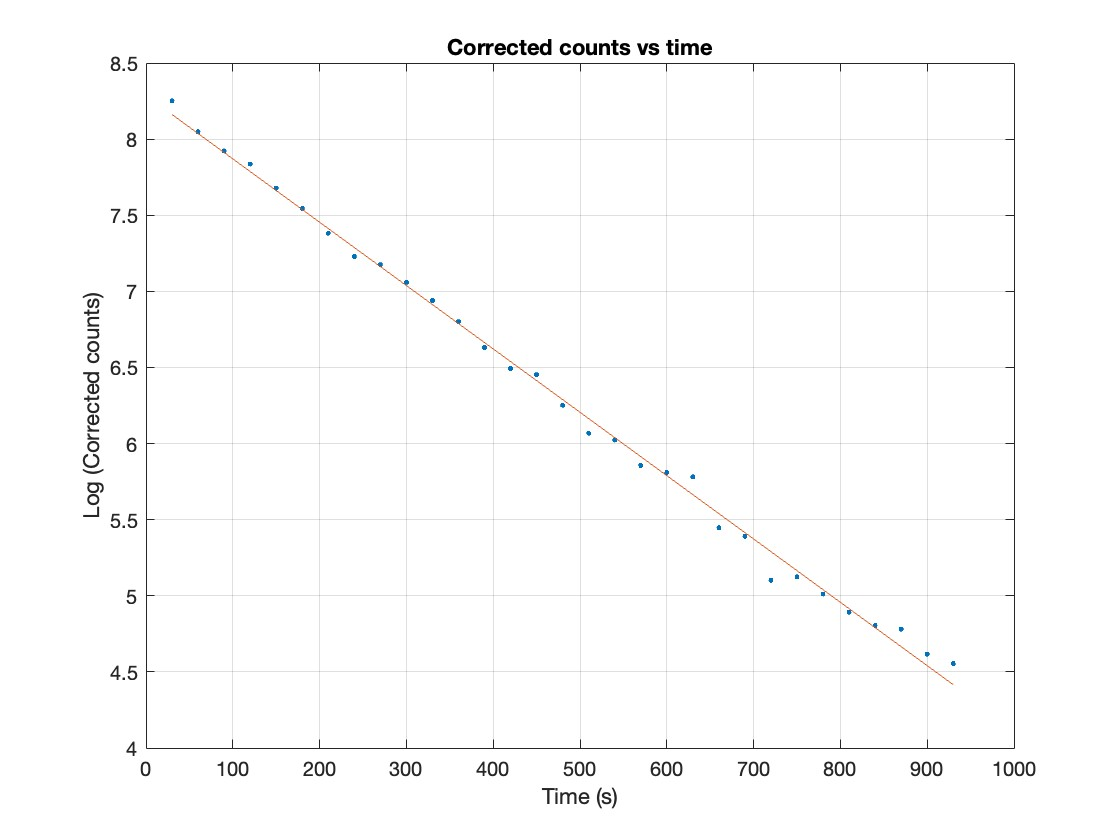
\includegraphics[width = \columnwidth]{Lab13_CorrectedCountsPlot.jpg}
    \caption{Plot of Ln(radiation counts), where the counts are  corrected for background radiation, as a function of time}
    \label{fig: CorrectedCountsPlot_Lab13}
\end{figure}


\begin{figure}
    \centering
    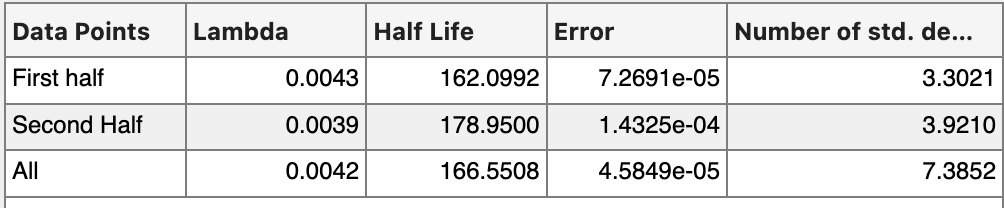
\includegraphics[width = \columnwidth]{Lab13_Table.png}
    \caption{Table of estimated half-life using different data points}
    \label{fig: Lab13_Table}
\end{figure}
Figure \ref{fig: ActivityPlot_Lab13} shows a plot of the natural log of radiation counts as a function of time. The data is fitted according to the equation $y = ax + b$ where $a = -0.0039$ and $b = 8.2320$ (with appropriate units). The R-squared value for the fit is 0.9942. Figure \ref{fig: CorrectedCountsPlot_Lab13} shows a plot of the natural log of corrected radiation counts as a function of time. The data is fitted according to the equation $y = ax + b$ where $a = -0.0042$ and $b = 8.2864$. The R-squared value for the fit is 0.9965.

Linear regression was applied to three different subsets of data: the first 15 points, the final 16 points, and the entire dataset. The regression for the first 15 points gave a linear fit where the slope is -0.0043 and the y-intercept is 8.3224. The standard error was found to be 0.0198. 
The regression for the final sixteen points gave a linear fit where the slope is -0.0039 and the y-intercept is 8.0751 (with appropriate units as seen in the plots). The standard error was found to be 0.1029. The regression for the entire data set gave a linear fit where the slope is -0.0042 and the y-intercept is 8.2864. The standard error was found to be 0.0252. 

The experimental rate of decay is  slope of the linear regression. Figure \ref{fig: Lab13_Table} shows the estimates for the half-life of the isotope and show the number of standard deviations away from the true value of 153 seconds the estimates are. 

\subsection{Conclusions}
The half-life was estimated to be 166.5 seconds. This is within 0.15 standard deviations of the true value of 153 seconds. 

\section{Conclusions}
The Geiger-Muller counter has been useful in a wide range of experiments that demonstrated the nature of radiation and helped the author gain a new understanding of radioactive decay. 



\section{Appendix A} 
All calculations and plots were done using MATLAB.  Links for MATLAB code here: \url{https://github.com/gdiaz001/RadiationLab}. 


\end{document}
